\documentclass{article}
\usepackage{graphicx}
\graphicspath{{../images/}}
\date{}
\title{USGS Earthquake Data Analysis}
\author{Akshay Yadav}
\begin{document}
	\maketitle
	\section{Abstract}
		This project is an attempt to build a R shiny application that downloads earthquake data between user defined dates from USGS database, processes the data into a convenient dataframes and displays using different types of visualizations. The earthquake records are displayed in form of histograms that show country and continent-wise distributions of earthquakes. The exact continent-wise locations of the earthquakes can also be viewed on an interactive world map. Two scatter plots, in a different tab, help to the explore relationship between the significance, depth and magnitude variables of the earthquakes. A slider widget is also provided which helps to filter-out less significant earthquakes for analysis. 
		
		\begin{figure}
			\fbox{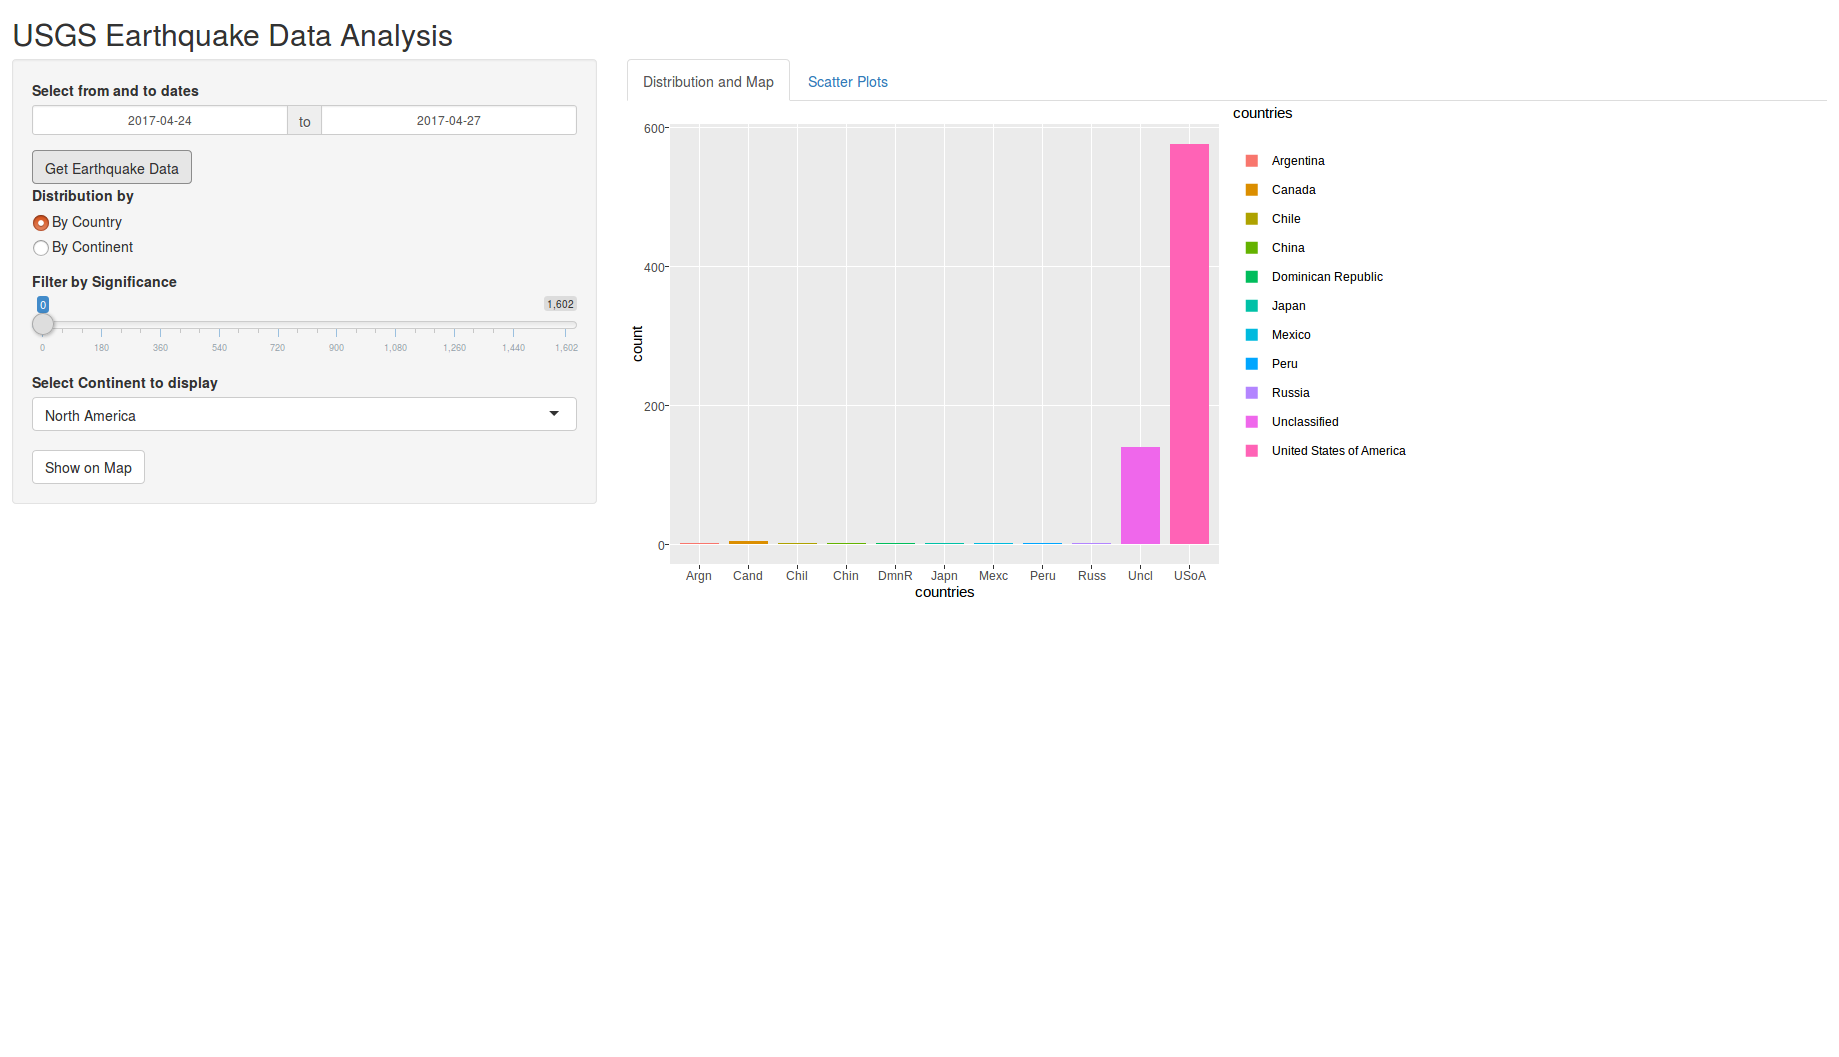
\includegraphics[width=\textwidth]{report_image1.png}}
			\caption{As an example, earthquake data from April, 24th 2017 to April, 27th 2017 is acquired. The country-wise distribution of earthquakes is automatically displayed}
		\end{figure}
		
		\begin{figure}
			\fbox{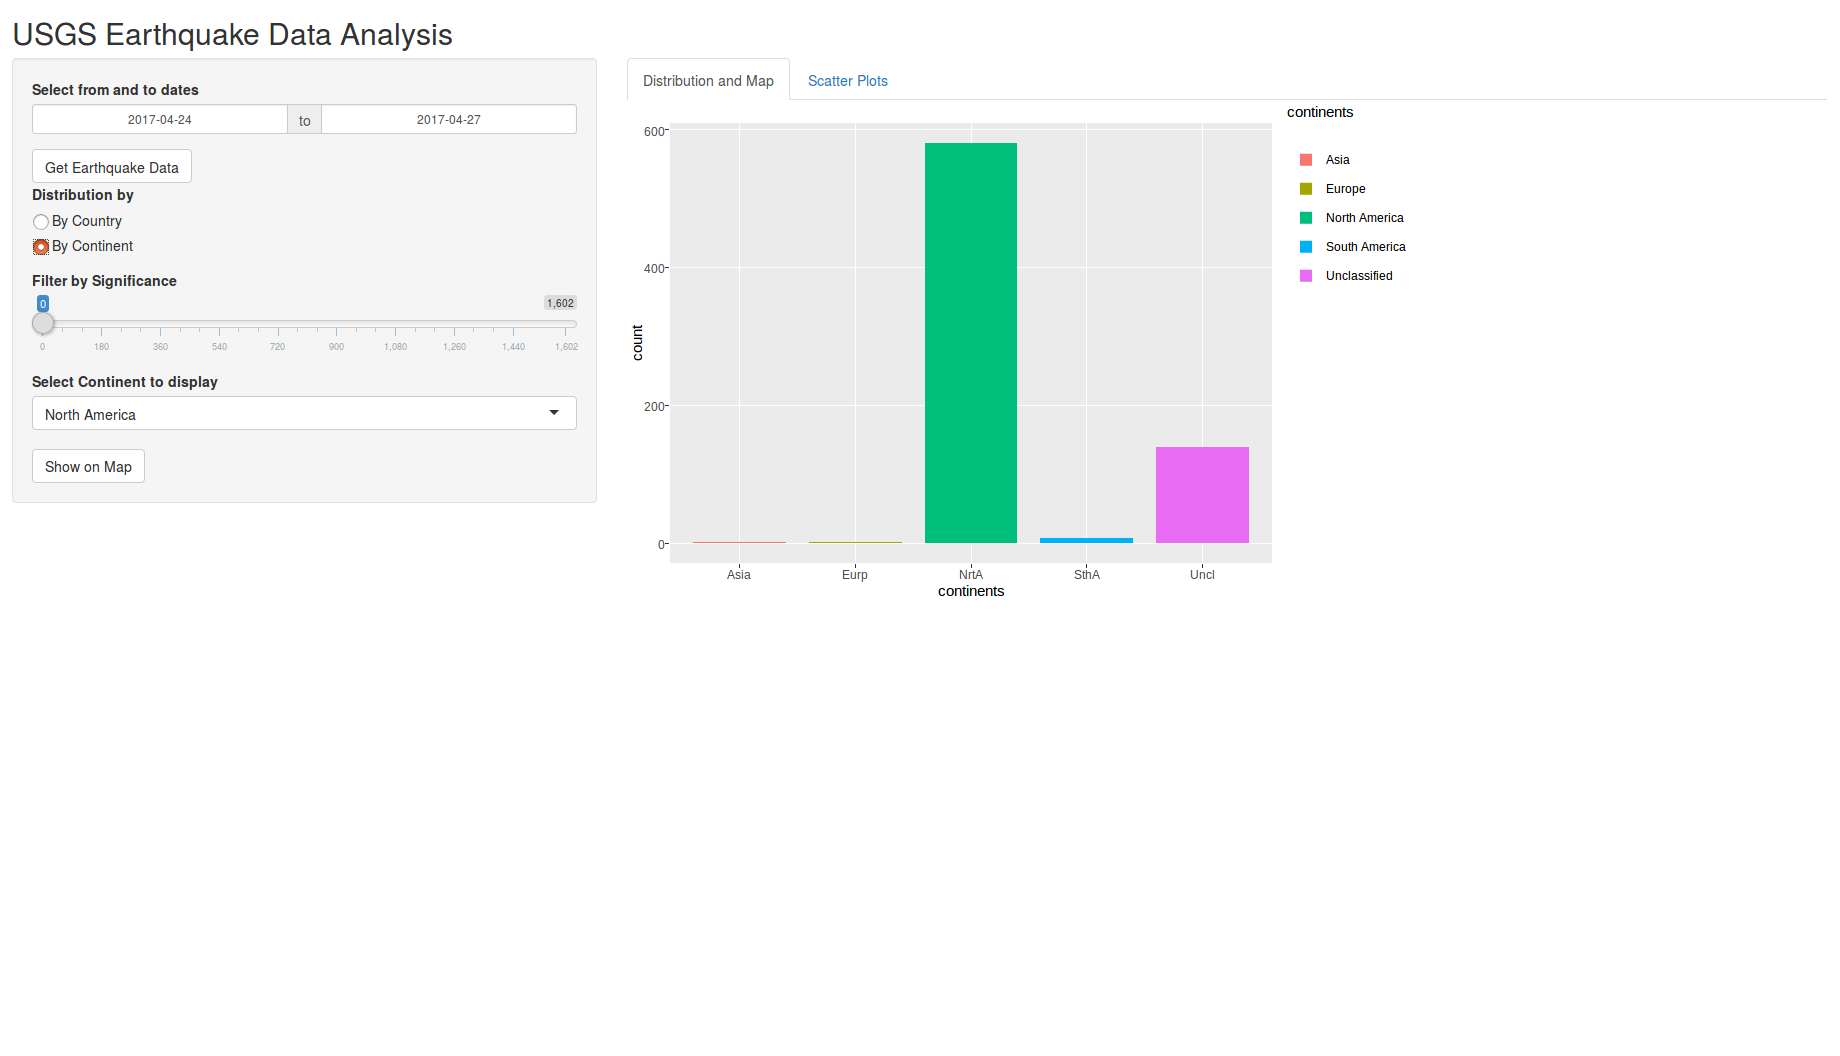
\includegraphics[width=\textwidth]{report_image2.png}}
			\caption{Using the "Distribution by" radio button the country-wise distribution histogram can be changed to continent-wise distribution histogram}
		\end{figure}
		
	\section{Introduction}
		The United States Geological Survey (USGS) is an agency that maintains records of the earthquakes that are detected in the US and around the world. These records are updated on a daily basis and can be accessed easily. Past and present records between any dates can be obtained through the agency webAPI service in JSON (geoJSON) or other convenient formats. In this project, I have attempted to build a R shiny application and related methods that download earthquake records between any specified dates and provide different visual representations of the records after processing the data. The following sections will describe the different application options and back-end data processing in a stepwise manner.
	
	\section{Data - Accessing, Format and Processing}
		The earthquake records from USGS database can be accessed using a customized webAPI URL which returns the earthquake data between specified dates. The user and can select the dates using a date-range selector widget which is displayed on application initialization. The "Get Earthquake Data" button, when clicked after selecting the desired dates, will initialize the data download and processing on the server-side. After the button is clicked, the custom URL to accomodate the user selected and dates is prepared and the earthquake records are downloaded from the agency database in the JSON format. The JSON contains information on different types information on earthquakes recorded between the specified dates in form of different qualitative and quantitative features. The JSON is processed using functions from the "jsonlite" package to obtain a list of three dataframes viz. feature, geometry and id. All the dataframes are column bound to obtain a single dataframe.
		
		\begin{figure}
			\fbox{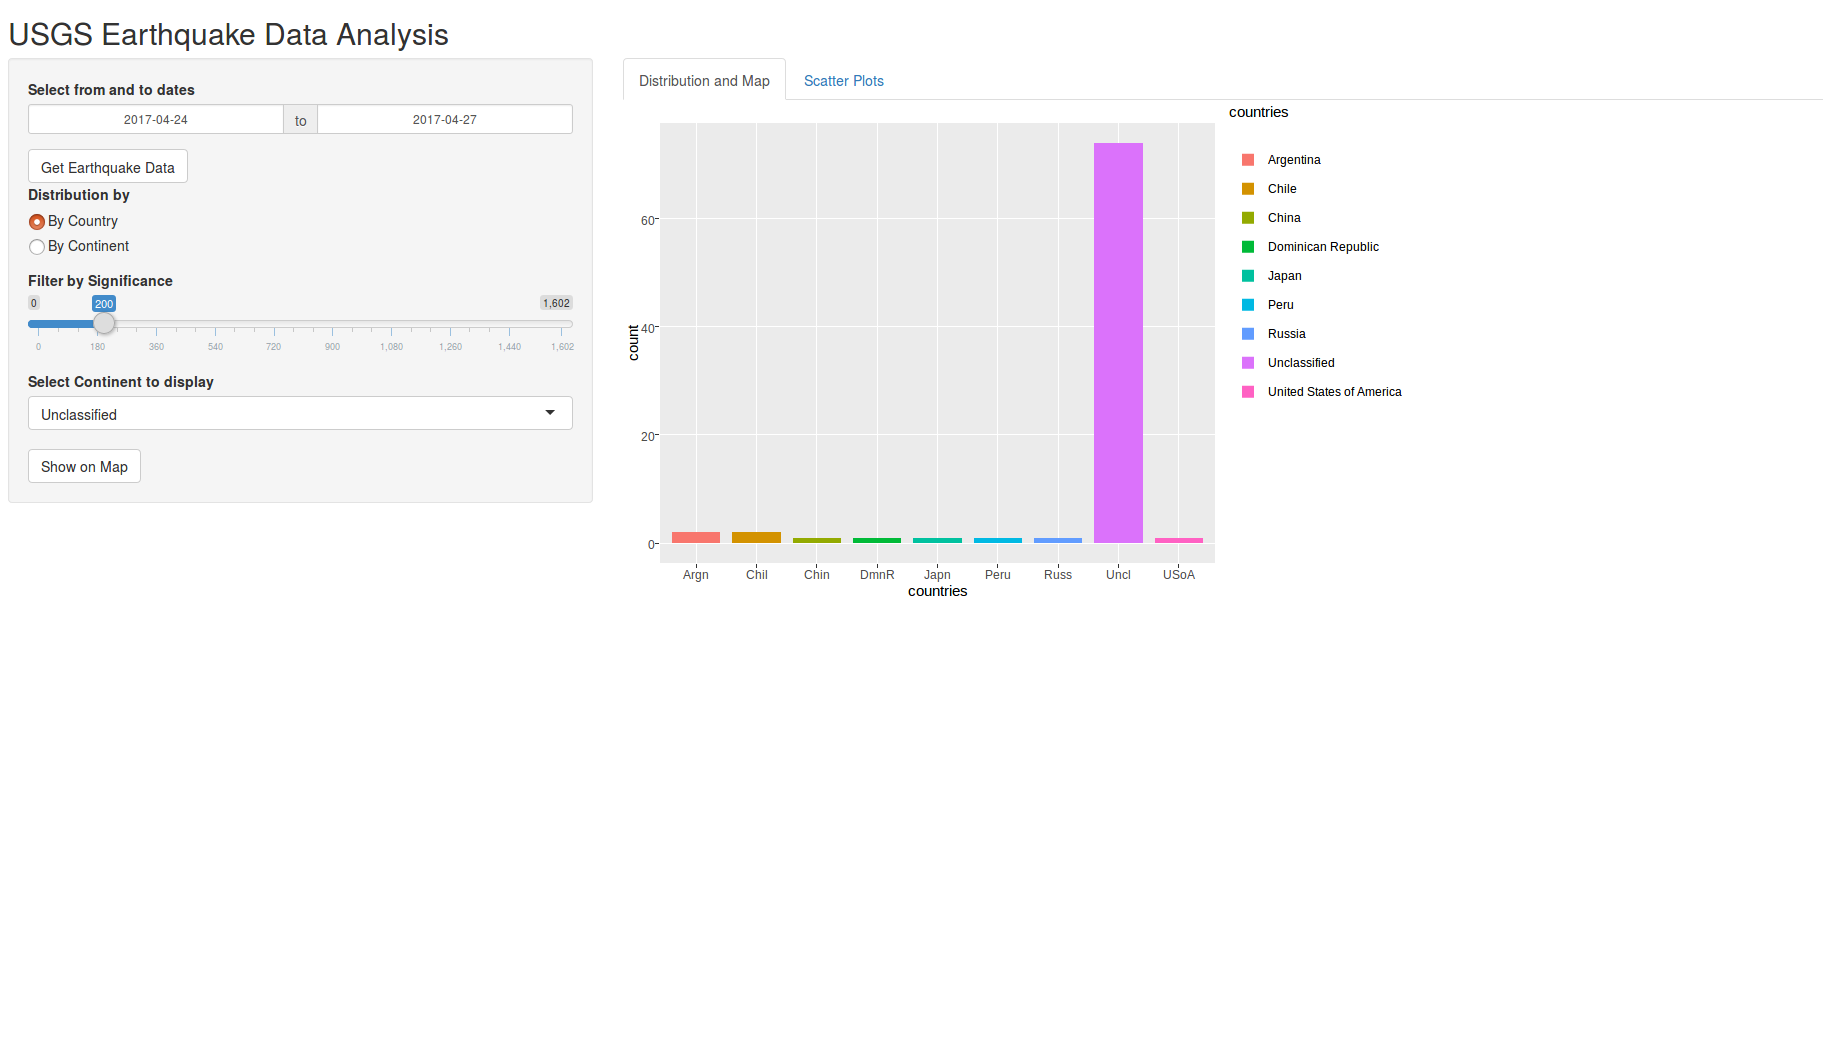
\includegraphics[width=\textwidth]{report_image3.png}}
			\caption{Earthquakes can be filtered on the significance values using the slider widget. We can see that most of the earthquakes from US are filtered out}
		\end{figure}
		
		\begin{figure}
			\fbox{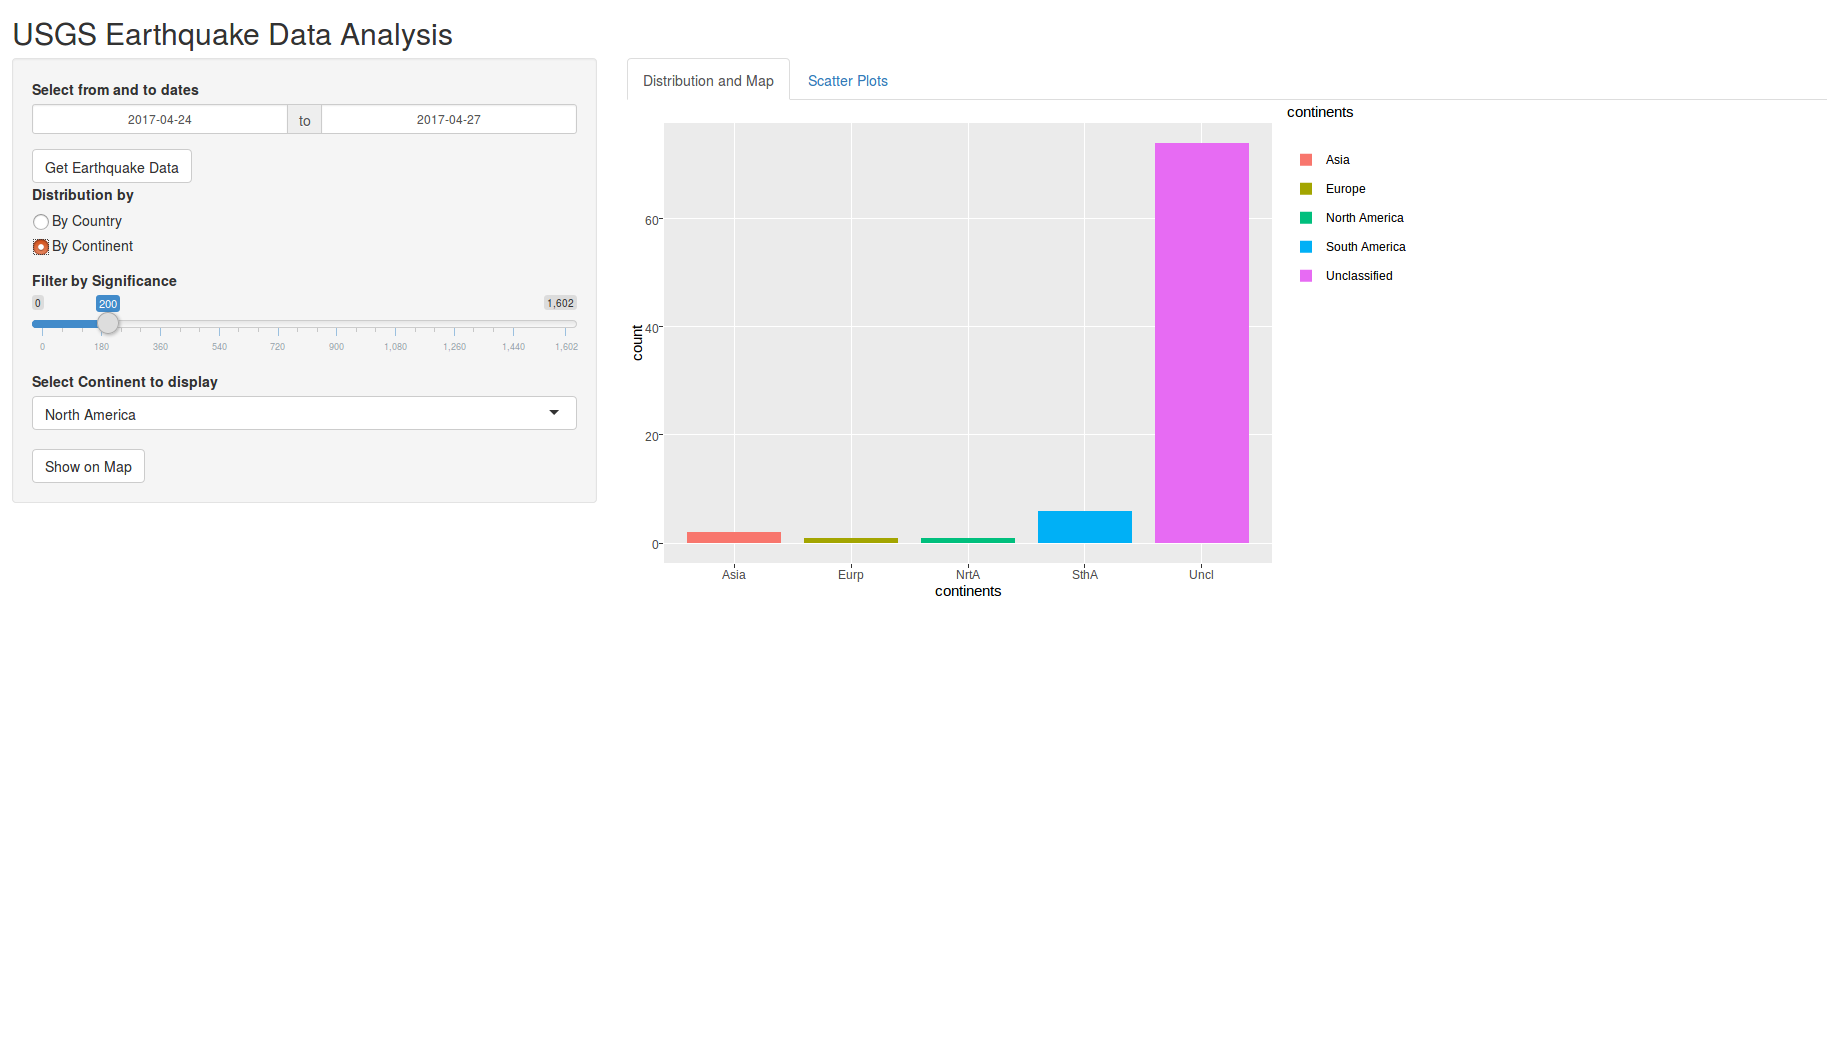
\includegraphics[width=\textwidth]{report_image4.png}}
			\caption{The effect of slider can also be seen on the continent-wise distribution. Most of the earthquakes from North American continent are filtered out}
		\end{figure}
		
		An additional processing step, included in this project, was to infer the names of the countries and continents for each earthquake in the data using the latitude and longitude coordinates in the feature dataframe. The "rworldmap" and "sp" packages were used for this purpose. The coordinate ranges for each country and continent were obtained using functions from "rworldmap" package and the actual earthquake coordinates were mapped to these coordinate ranges using functions from the spacial "sp" packages. Two new columns specifying the country and continent names for the earthquakes were added to the earthquake records dataframe obtained earlier to get the final processed dataframe. The earthquakes detected in oceans and disputed territories were marked as "Unclassfied" in the countries or continent columns.
		
	\section{Data Visualization}
		
		\begin{figure}
			\fbox{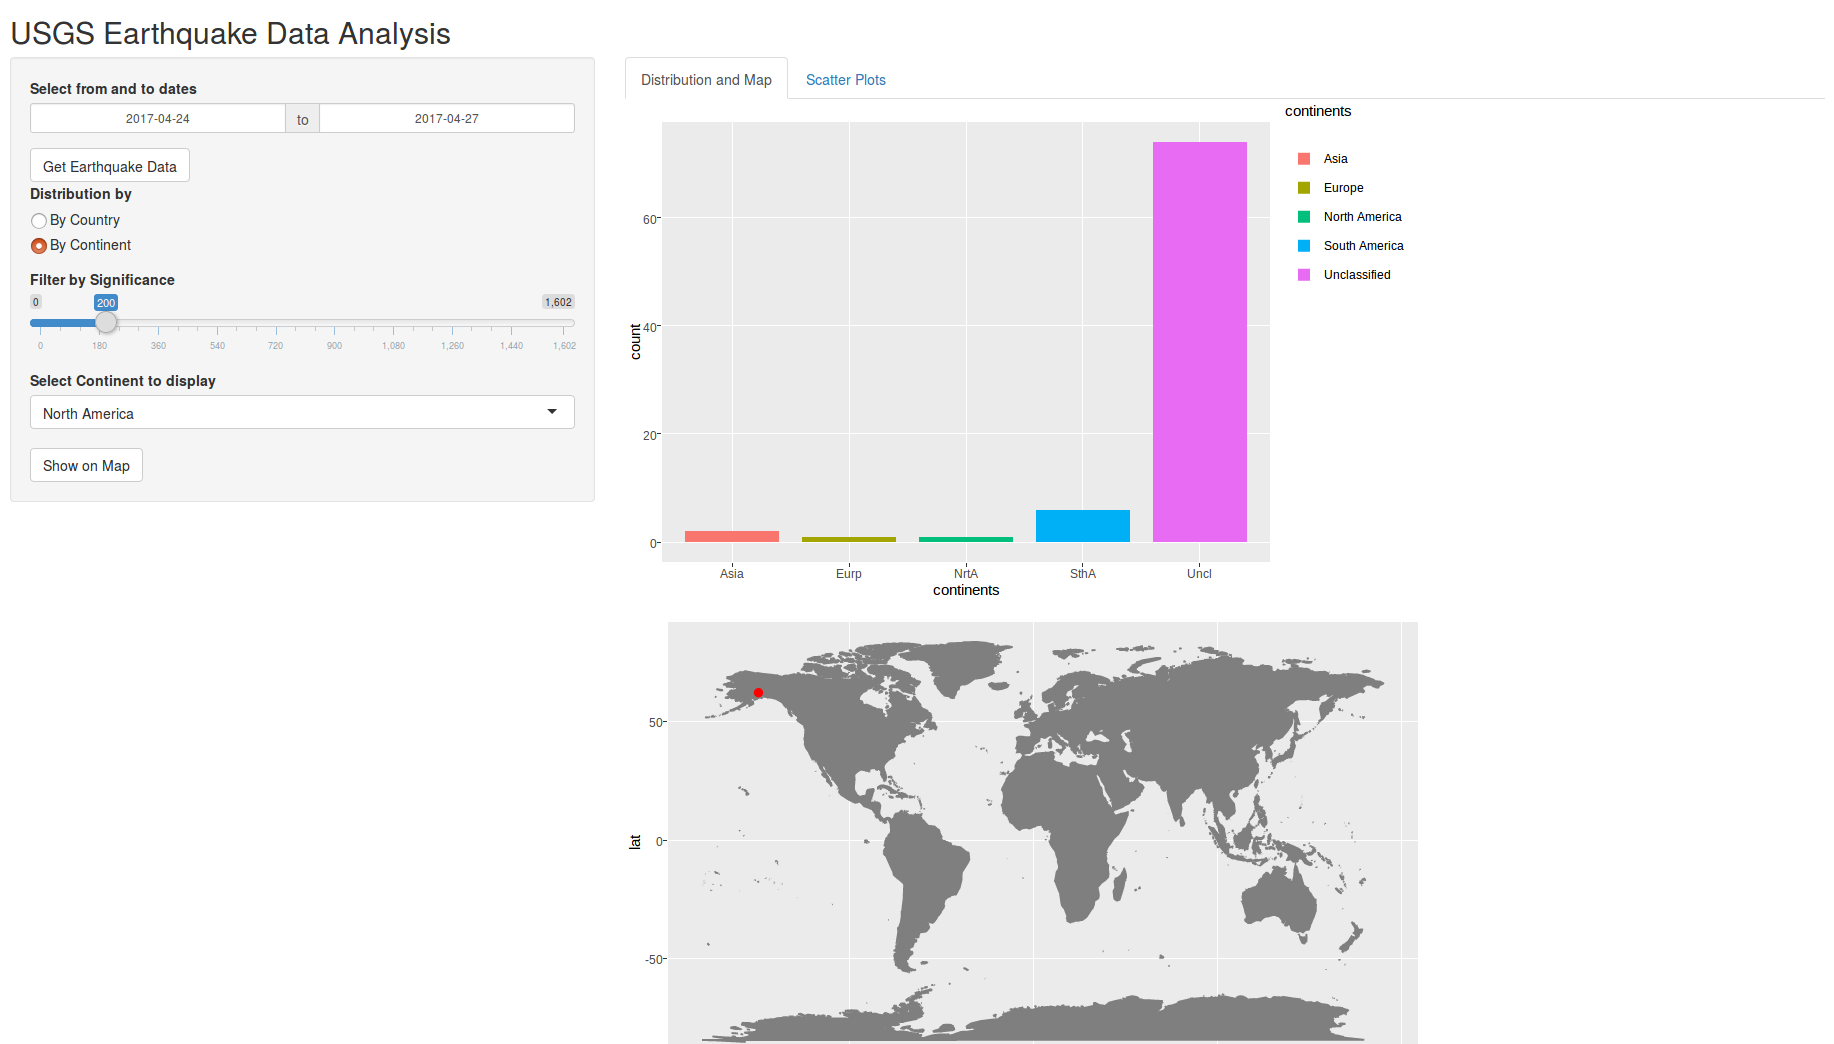
\includegraphics[width=\textwidth]{report_image5.png}}
			\caption{The exact location of earthquake can be viewed on a map by selecting a continent name from the drop down and clicking on the "Show on Map" button}
		\end{figure}
		
		\begin{figure}
			\fbox{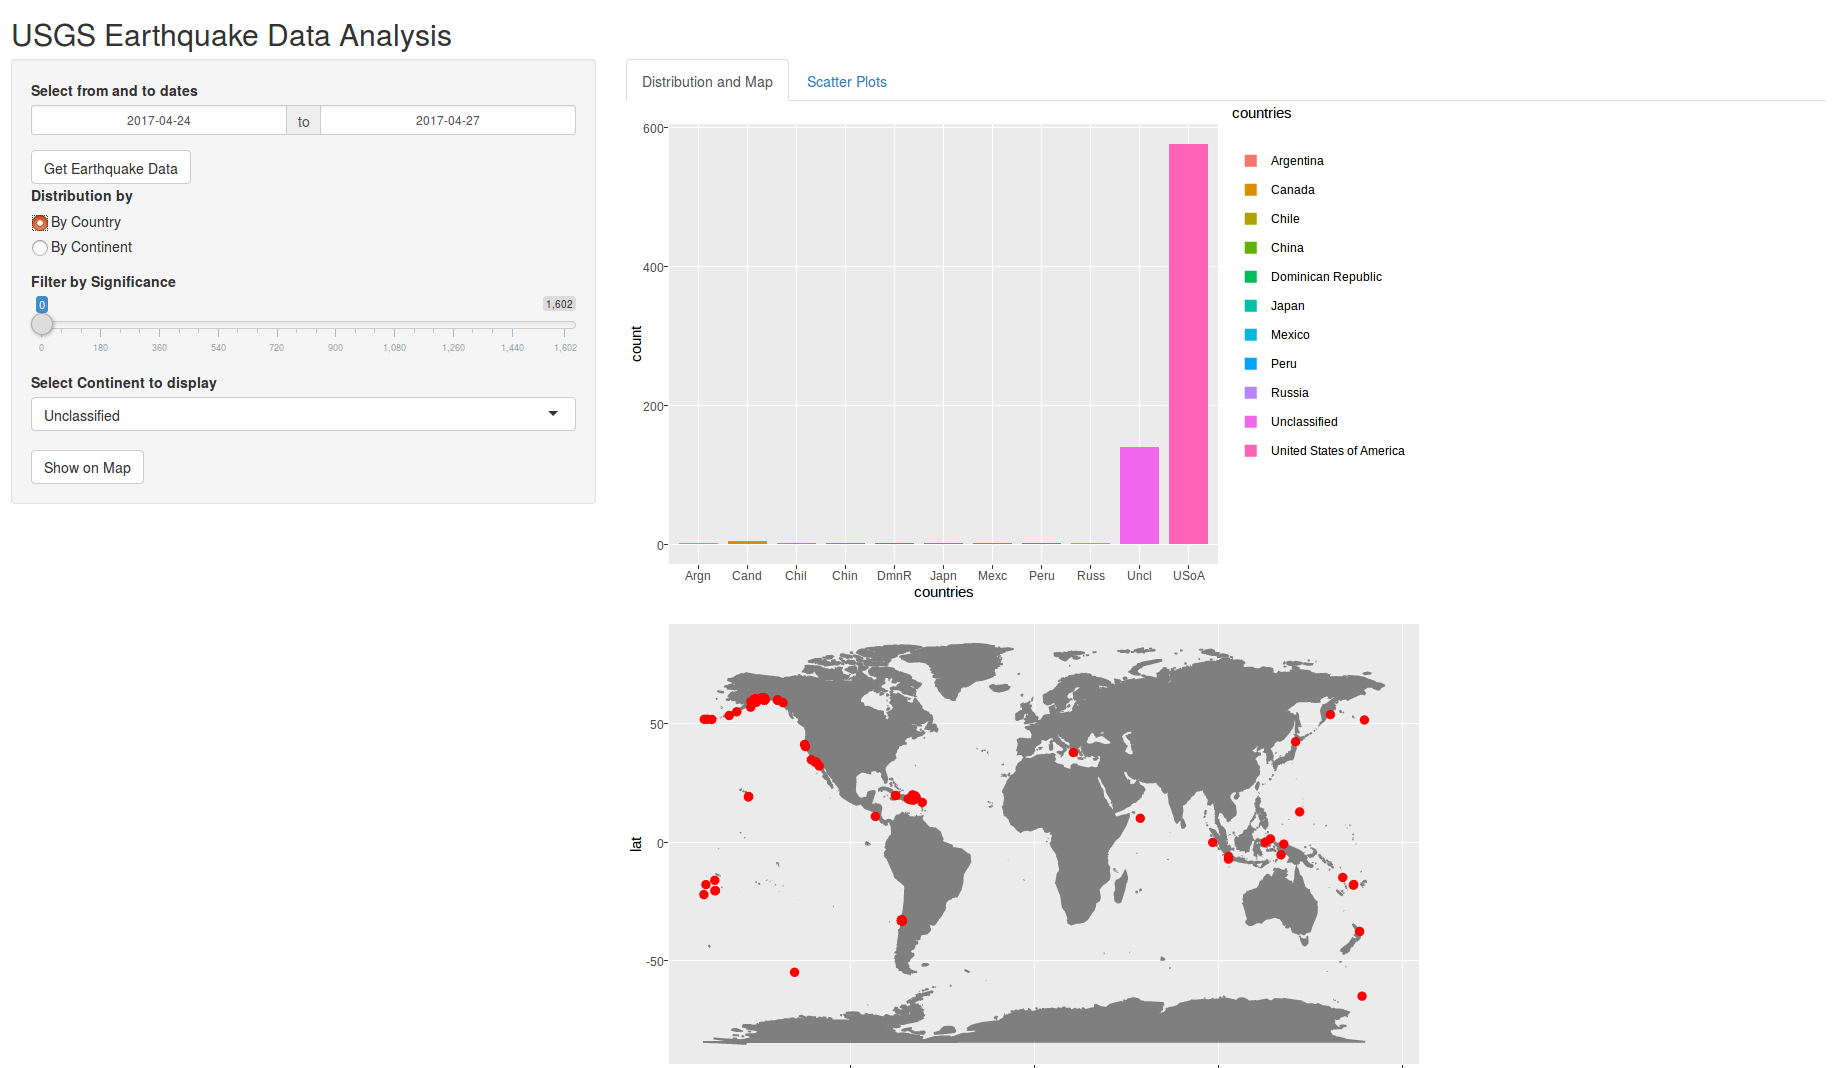
\includegraphics[width=\textwidth]{report_image6.png}}
			\caption{Selecting the "Unclassified" option from the continent list will plot all the earthquakes that occur in oceans}
		\end{figure}
		
		When the data processing is complete, a histogram that shows a country-wise distribution (Figure 1) of earthquakes is displayed automatically, along with a radio button widget below the "Get Earthquake Data" button. The radio button widget has two options and can be used to change the histogram to show continent-wise distribution of the earthquakes (Figure 2). The histograms are interactive and can be used to show/hide desired countries or continents in the histograms.
			
		One of the most important quantitative features for each earthquake record is the "significance" value of the earthquakes. This value is assigned to the earthquakes by USGS and is function of other earthquake variables such as magnitude, maximum MMI, number of felt reports and estimated impact. The significance value therefore can tell us how significant the earthquake was in a more complete sense. In this application, the user can used a slider widget displayed below the radio button to filter out less significant earthquakes (Figure 3,4). The default value of the slider is set to zero so that no records are filtered out by default. The effect of slider widget is automatically reflected in country-wise and continent-wise distribution histograms.
		
		The exact location of earthquakes can be viewed on a world map (Figure 5,6) using the drop-down and "Show on Map" button widgets, displayed below the slider widget. Selecting the desired continent from the drop down and clicking the "Show on Map" button will display the earthquakes related to the selected continent on an interactive world map. Selecting a different continent and clicking on the button will update the map to show the earthquakes related to newly selected continent. The effect of the slider widget is also reflected automatically on the map.
		
		\begin{figure}
			\fbox{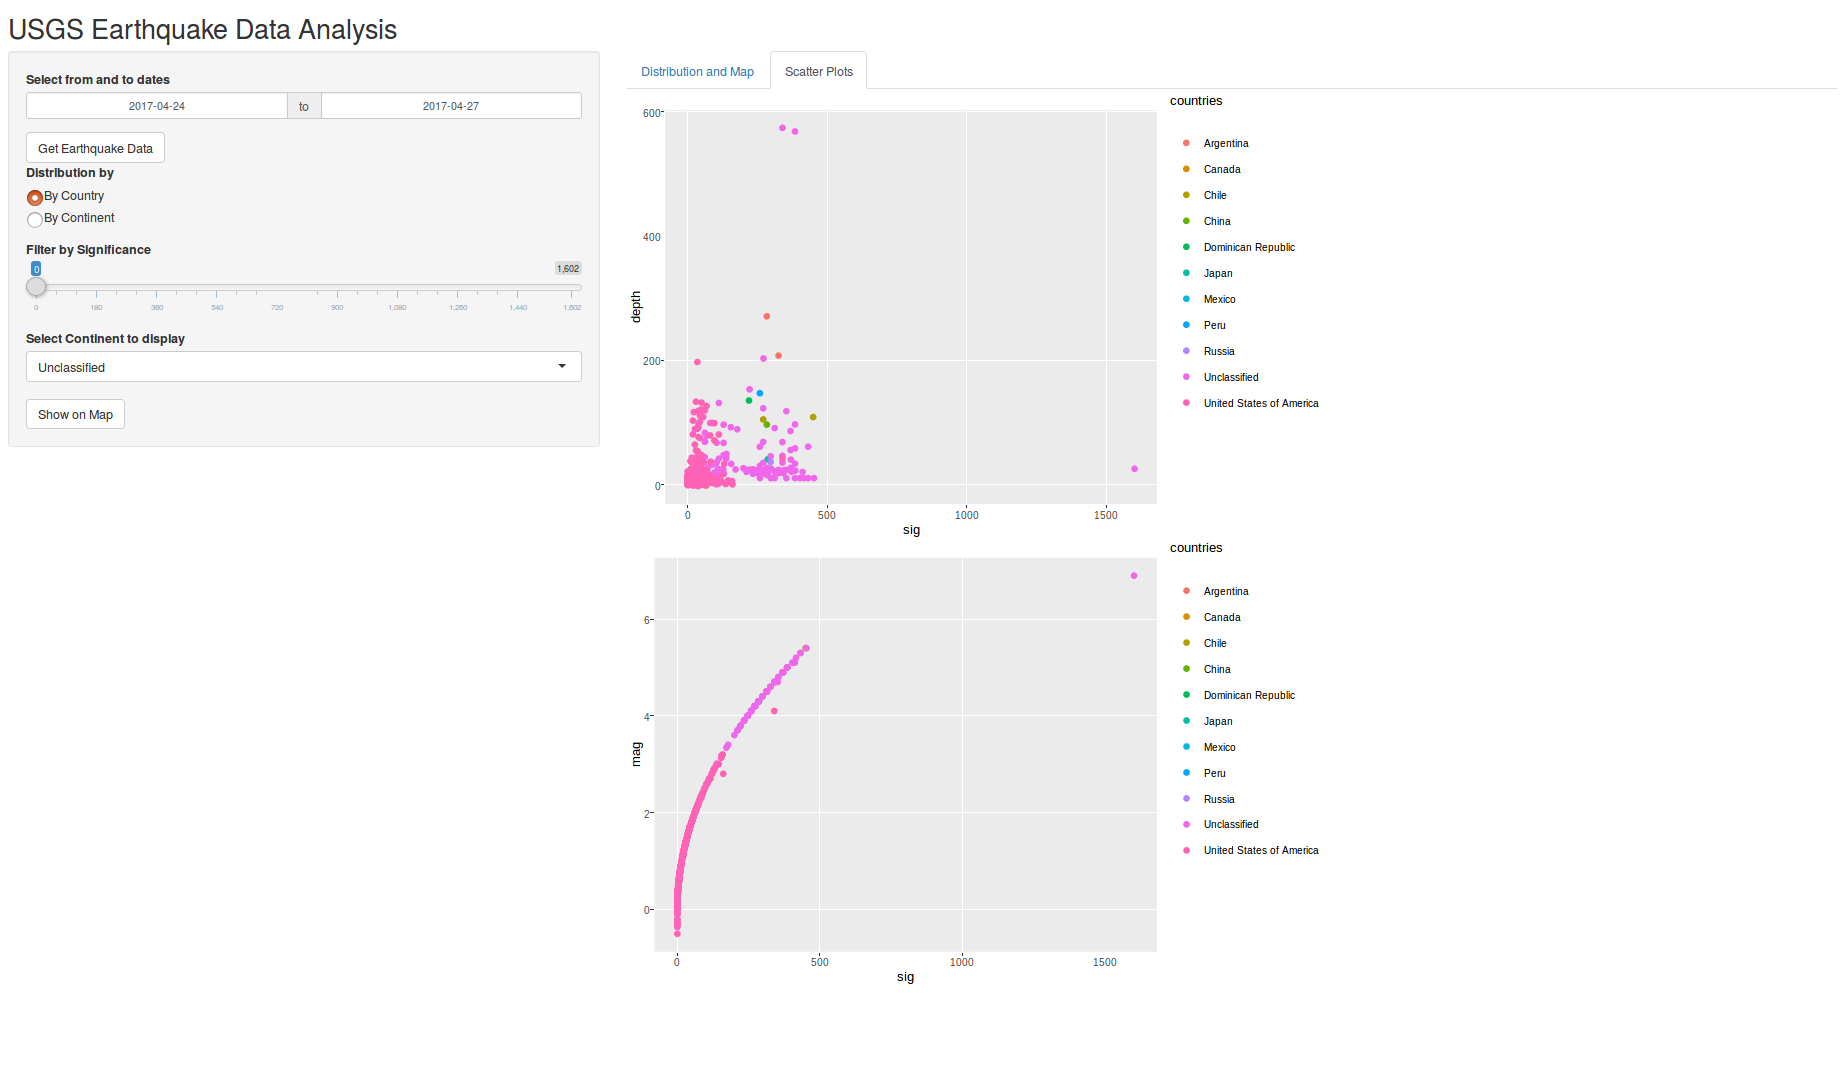
\includegraphics[width=\textwidth]{report_image7.png}}
			\caption{The Significance v/s Depth and Significance v/s Magnitude scatter plots show the relationship between the variables}
		\end{figure}
		
		In a second "Scatter Plot" tab, two interactive scatter plots (Figure 7) that show relationship between the signficance v/s depth values and significance v/s the magnitude values are displayed. The points are colored according to country or continent names (according to selection in the radio button wigdet) and can be modified to show/hide points related to one or more countries or continents. Here too, the effect of using the significance slider widget is automatically reflected in both the scatter plots.
	
\end{document}